% Options for packages loaded elsewhere
\PassOptionsToPackage{unicode}{hyperref}
\PassOptionsToPackage{hyphens}{url}
\PassOptionsToPackage{dvipsnames,svgnames,x11names}{xcolor}
%
\documentclass[a4paper,12pt]{article}
\usepackage[notransparent]{svg}
\usepackage[utf8]{inputenc}
\usepackage[lmargin=3cm,tmargin=3cm,rmargin=2cm,bmargin=2cm]{geometry}
\usepackage{fancyhdr}
\usepackage{orcidlink}
\fancyhf{}
\fancyhead[R]{\thepage}
\renewcommand{\headrulewidth}{0pt}
\usepackage[onehalfspacing]{setspace}
\usepackage{blindtext}
\usepackage[T1]{fontenc}
% \usepackage[brazil]{babel}
\usepackage[document]{ragged2e}
\usepackage{pdflscape}
\usepackage{pdfpages}
\usepackage{float}
\usepackage{changepage}

\usepackage{graphicx, xcolor, comment, enumerate, multirow, multicol}
\usepackage{indentfirst}

\usepackage{amsfonts, amsthm, amsmath, amssymb, dsfont, mathtools}
\usepackage{tikz, tkz-base, tkz-fct}
\usepackage[style=abnt]{biblatex}

\usepackage{titlesec}
\usepackage{adjustbox}
\usepackage[skip=5pt, indent=15pt]{parskip}

\titleformat{\section}
{\normalsize\bfseries}{\thesection.}{1em}{}
\titleformat{\subsection}
{\normalsize}{\thesubsection.}{1em}{}
\titleformat{\subsubsection}
{\normalsize}{\thesubsubsection.}{1em}{}

\newcommand{\PR}[1]{\ensuremath{\left[#1\right]}}
\newcommand{\PC}[1]{\ensuremath{\left(#1\right)}}
\newcommand{\chav}[1]{\ensuremath{\left\{#1\right\}}}
\newcommand{\system}[1]{\ensuremath{\left\{#1\right}}
\newcommand{\floor}[1]{\ensuremath{\left \lfloor #1\right \rfloor}}
\newcommand{\FontTable}[1]{\vspace{-\baselineskip}\begin{footnotesize}#1\end{footnotesize}}

% Citacao direta com mais de 3 linhas - ABNT NBR 10520/2002 - 5.3
\newlength{\ABNTEXcitacaorecuo}% recuo de 4 cm da margem esquerda
\setlength{\ABNTEXcitacaorecuo}{4cm}
\newcommand{\ABNTEXfontereduzida}{\footnotesize}
\newenvironment*{citacao}[1][default]{%
   \list{}%
   \ABNTEXfontereduzida%
   \addtolength{\leftskip}{\ABNTEXcitacaorecuo}%
   \item[]%
   \singlespacing
   \ifthenelse{\not\equal{#1}{default}}{\itshape\selectlanguage{#1}}{}%
 }{%
   \endlist}%
% ---


% Citacao direta com mais de 3 linhas - ABNT NBR 10520/2002 - 5.3
\newlength{\aprovacao}% recuo de 4 cm da margem esquerda
\setlength{\aprovacao}{10.5cm}
\newcommand{\aprovacaofonte}{\normalsize}
\newenvironment*{citacao2}[1][default]{%
   \list{}%
   \aprovacaofonte%
   \addtolength{\leftskip}{\aprovacao}%
   \item[]%
   \singlespacing
   \justify
   \ifthenelse{\not\equal{#1}{default}}{\itshape\selectlanguage{#1}}{}%
 }{%
   \endlist}%
% ---


\newcommand{\fig}[4]{%
  \begin{figure}[H]
    \centering
    \caption{#1}
    \label{#2}
    \includegraphics{#3}
    
    \vspace{0.5cm}
    
    \begin{footnotesize}
      Fonte: #4
    \end{footnotesize}
  \end{figure}
}

\newcommand{\quadro}[4]{%
  \renewcommand{\figurename}{Quadro}
  \setcounter{figure}{0}
  \begin{figure}[H]
    \captionsetup{list=no}
    \centering
    \caption{#1}
    \label{#2}
    \includegraphics{#3}
    
    \vspace{0.5cm}
    
    \begin{footnotesize}
      Fonte: #4
    \end{footnotesize}
  \end{figure}
}

\newenvironment{invisible}{\color{white}}{}

\usepackage{amsmath,amssymb}
\usepackage{iftex}
\ifPDFTeX
  \usepackage[T1]{fontenc}
  \usepackage[utf8]{inputenc}
  \usepackage{textcomp} % provide euro and other symbols
\else % if luatex or xetex
  \usepackage{unicode-math}
  \defaultfontfeatures{Scale=MatchLowercase}
  \defaultfontfeatures[\rmfamily]{Ligatures=TeX,Scale=1}
\fi
\usepackage{lmodern}
\ifPDFTeX\else  
    % xetex/luatex font selection
  \setmainfont[]{Times New Roman}
\fi
% Use upquote if available, for straight quotes in verbatim environments
\IfFileExists{upquote.sty}{\usepackage{upquote}}{}
\IfFileExists{microtype.sty}{% use microtype if available
  \usepackage[]{microtype}
  \UseMicrotypeSet[protrusion]{basicmath} % disable protrusion for tt fonts
}{}
\makeatletter
\@ifundefined{KOMAClassName}{% if non-KOMA class
  \IfFileExists{parskip.sty}{%
    \usepackage{parskip}
  }{% else
    \setlength{\parindent}{0pt}
    \setlength{\parskip}{6pt plus 2pt minus 1pt}}
}{% if KOMA class
  \KOMAoptions{parskip=half}}
\makeatother
\usepackage{xcolor}
\setlength{\emergencystretch}{3em} % prevent overfull lines
\setcounter{secnumdepth}{5}
% Make \paragraph and \subparagraph free-standing
\ifx\paragraph\undefined\else
  \let\oldparagraph\paragraph
  \renewcommand{\paragraph}[1]{\oldparagraph{#1}\mbox{}}
\fi
\ifx\subparagraph\undefined\else
  \let\oldsubparagraph\subparagraph
  \renewcommand{\subparagraph}[1]{\oldsubparagraph{#1}\mbox{}}
\fi

\usepackage{color}
\usepackage{fancyvrb}
\newcommand{\VerbBar}{|}
\newcommand{\VERB}{\Verb[commandchars=\\\{\}]}
\DefineVerbatimEnvironment{Highlighting}{Verbatim}{commandchars=\\\{\}}
% Add ',fontsize=\small' for more characters per line
\newenvironment{Shaded}{}{}
\newcommand{\AlertTok}[1]{\textcolor[rgb]{0.58,0.85,0.30}{\textbf{\colorbox[rgb]{0.30,0.12,0.14}{#1}}}}
\newcommand{\AnnotationTok}[1]{\textcolor[rgb]{0.31,0.63,0.31}{#1}}
\newcommand{\AttributeTok}[1]{\textcolor[rgb]{0.65,0.15,0.64}{#1}}
\newcommand{\BaseNTok}[1]{\textcolor[rgb]{0.60,0.41,0.00}{#1}}
\newcommand{\BuiltInTok}[1]{\textcolor[rgb]{0.65,0.15,0.64}{#1}}
\newcommand{\CharTok}[1]{\textcolor[rgb]{0.31,0.63,0.31}{#1}}
\newcommand{\CommentTok}[1]{\textcolor[rgb]{0.63,0.63,0.65}{\textit{#1}}}
\newcommand{\CommentVarTok}[1]{\textcolor[rgb]{0.89,0.34,0.29}{\textit{#1}}}
\newcommand{\ConstantTok}[1]{\textcolor[rgb]{0.60,0.41,0.00}{#1}}
\newcommand{\ControlFlowTok}[1]{\textcolor[rgb]{0.65,0.15,0.64}{#1}}
\newcommand{\DataTypeTok}[1]{\textcolor[rgb]{0.65,0.15,0.64}{#1}}
\newcommand{\DecValTok}[1]{\textcolor[rgb]{0.60,0.41,0.00}{#1}}
\newcommand{\DocumentationTok}[1]{\textcolor[rgb]{0.89,0.34,0.29}{#1}}
\newcommand{\ErrorTok}[1]{\textcolor[rgb]{0.96,0.28,0.28}{\underline{#1}}}
\newcommand{\ExtensionTok}[1]{\textcolor[rgb]{0.25,0.47,0.95}{\textbf{#1}}}
\newcommand{\FloatTok}[1]{\textcolor[rgb]{0.60,0.41,0.00}{#1}}
\newcommand{\FunctionTok}[1]{\textcolor[rgb]{0.25,0.47,0.95}{#1}}
\newcommand{\ImportTok}[1]{\textcolor[rgb]{0.31,0.63,0.31}{#1}}
\newcommand{\InformationTok}[1]{\textcolor[rgb]{0.77,0.36,0.00}{#1}}
\newcommand{\KeywordTok}[1]{\textcolor[rgb]{0.65,0.15,0.64}{#1}}
\newcommand{\NormalTok}[1]{\textcolor[rgb]{0.22,0.23,0.26}{#1}}
\newcommand{\OperatorTok}[1]{\textcolor[rgb]{0.65,0.15,0.64}{#1}}
\newcommand{\OtherTok}[1]{\textcolor[rgb]{0.15,0.68,0.38}{#1}}
\newcommand{\PreprocessorTok}[1]{\textcolor[rgb]{0.65,0.15,0.64}{#1}}
\newcommand{\RegionMarkerTok}[1]{\textcolor[rgb]{0.16,0.50,0.73}{\colorbox[rgb]{0.08,0.19,0.26}{#1}}}
\newcommand{\SpecialCharTok}[1]{\textcolor[rgb]{0.00,0.52,0.74}{#1}}
\newcommand{\SpecialStringTok}[1]{\textcolor[rgb]{0.85,0.27,0.33}{#1}}
\newcommand{\StringTok}[1]{\textcolor[rgb]{0.31,0.63,0.31}{#1}}
\newcommand{\VariableTok}[1]{\textcolor[rgb]{0.89,0.34,0.29}{#1}}
\newcommand{\VerbatimStringTok}[1]{\textcolor[rgb]{0.85,0.27,0.33}{#1}}
\newcommand{\WarningTok}[1]{\textcolor[rgb]{0.85,0.27,0.33}{#1}}

\providecommand{\tightlist}{%
  \setlength{\itemsep}{0pt}\setlength{\parskip}{0pt}}\usepackage{longtable,booktabs,array}
\usepackage{calc} % for calculating minipage widths
% Correct order of tables after \paragraph or \subparagraph
\usepackage{etoolbox}
\makeatletter
\patchcmd\longtable{\par}{\if@noskipsec\mbox{}\fi\par}{}{}
\makeatother
% Allow footnotes in longtable head/foot
\IfFileExists{footnotehyper.sty}{\usepackage{footnotehyper}}{\usepackage{footnote}}
\makesavenoteenv{longtable}
\usepackage{graphicx}
\makeatletter
\def\maxwidth{\ifdim\Gin@nat@width>\linewidth\linewidth\else\Gin@nat@width\fi}
\def\maxheight{\ifdim\Gin@nat@height>\textheight\textheight\else\Gin@nat@height\fi}
\makeatother
% Scale images if necessary, so that they will not overflow the page
% margins by default, and it is still possible to overwrite the defaults
% using explicit options in \includegraphics[width, height, ...]{}
\setkeys{Gin}{width=\maxwidth,height=\maxheight,keepaspectratio}
% Set default figure placement to htbp
\makeatletter
\def\fps@figure{htbp}
\makeatother
\newlength{\cslhangindent}
\setlength{\cslhangindent}{1.5em}
\newlength{\csllabelwidth}
\setlength{\csllabelwidth}{3em}
\newlength{\cslentryspacingunit} % times entry-spacing
\setlength{\cslentryspacingunit}{\parskip}
\newenvironment{CSLReferences}[2] % #1 hanging-ident, #2 entry spacing
 {% don't indent paragraphs
  \setlength{\parindent}{0pt}
  % turn on hanging indent if param 1 is 1
  \ifodd #1
  \let\oldpar\par
  \def\par{\hangindent=\cslhangindent\oldpar}
  \fi
  % set entry spacing
  \setlength{\parskip}{#2\cslentryspacingunit}
 }%
 {}
\usepackage{calc}
\newcommand{\CSLBlock}[1]{#1\hfill\break}
\newcommand{\CSLLeftMargin}[1]{\parbox[t]{\csllabelwidth}{#1}}
\newcommand{\CSLRightInline}[1]{\parbox[t]{\linewidth - \csllabelwidth}{#1}\break}
\newcommand{\CSLIndent}[1]{\hspace{\cslhangindent}#1}

\DefineVerbatimEnvironment{Highlighting}{Verbatim}{commandchars=\\\{\},fontsize=\footnotesize}
\makeatletter
\makeatother
\makeatletter
\makeatother
\makeatletter
\@ifpackageloaded{caption}{}{\usepackage{caption}}
\AtBeginDocument{%
\ifdefined\contentsname
  \renewcommand*\contentsname{Índice}
\else
  \newcommand\contentsname{Índice}
\fi
\ifdefined\listfigurename
  \renewcommand*\listfigurename{Lista de Figuras}
\else
  \newcommand\listfigurename{Lista de Figuras}
\fi
\ifdefined\listtablename
  \renewcommand*\listtablename{Lista de Tabelas}
\else
  \newcommand\listtablename{Lista de Tabelas}
\fi
\ifdefined\figurename
  \renewcommand*\figurename{Figura}
\else
  \newcommand\figurename{Figura}
\fi
\ifdefined\tablename
  \renewcommand*\tablename{Tabela}
\else
  \newcommand\tablename{Tabela}
\fi
}
\@ifpackageloaded{float}{}{\usepackage{float}}
\floatstyle{ruled}
\@ifundefined{c@chapter}{\newfloat{codelisting}{h}{lop}}{\newfloat{codelisting}{h}{lop}[chapter]}
\floatname{codelisting}{Listagem}
\newcommand*\listoflistings{\listof{codelisting}{Lista de Listagens}}
\makeatother
\makeatletter
\@ifpackageloaded{caption}{}{\usepackage{caption}}
\@ifpackageloaded{subcaption}{}{\usepackage{subcaption}}
\makeatother
\makeatletter
\@ifpackageloaded{tcolorbox}{}{\usepackage[skins,breakable]{tcolorbox}}
\makeatother
\makeatletter
\@ifundefined{shadecolor}{\definecolor{shadecolor}{rgb}{.97, .97, .97}}
\makeatother
\makeatletter
\makeatother
\makeatletter
\makeatother
\ifLuaTeX
\usepackage[bidi=basic]{babel}
\else
\usepackage[bidi=default]{babel}
\fi
\babelprovide[main,import]{brazilian}
% get rid of language-specific shorthands (see #6817):
\let\LanguageShortHands\languageshorthands
\def\languageshorthands#1{}
\ifLuaTeX
  \usepackage{selnolig}  % disable illegal ligatures
\fi
\IfFileExists{bookmark.sty}{\usepackage{bookmark}}{\usepackage{hyperref}}
\IfFileExists{xurl.sty}{\usepackage{xurl}}{} % add URL line breaks if available
\urlstyle{same} % disable monospaced font for URLs
\hypersetup{
  pdftitle={MÍNIMOS QUADRADOS ORDINÁRIOS: UMA APLICAÇÃO NA ANÁLISE DAS QUESTÕES INSTITUCIONAIS DE MUNICÍPIOS BRASILEIROS},
  pdfauthor={Flávio Hugo Pangracio Silva; Guilherme Gomes Ferreira},
  pdflang={pt-BR},
  colorlinks=true,
  linkcolor={black},
  filecolor={Maroon},
  citecolor={Blue},
  urlcolor={Blue},
  pdfcreator={LaTeX via pandoc}}

\title{MÍNIMOS QUADRADOS ORDINÁRIOS: UMA APLICAÇÃO NA ANÁLISE DAS
QUESTÕES INSTITUCIONAIS DE MUNICÍPIOS BRASILEIROS}
\author{Flávio Hugo Pangracio Silva \and Guilherme Gomes Ferreira}
\date{}

\begin{document}
% Capa
\thispagestyle{empty}
\pagenumbering{roman}

\begin{center}
UNIVERSIDADE FEDERAL DE MINAS GERAIS
\end{center}


\vspace{3.5cm}

\begin{center}
    \textbf{MÍNIMOS QUADRADOS ORDINÁRIOS: UMA APLICAÇÃO NA ANÁLISE DAS
QUESTÕES INSTITUCIONAIS DE MUNICÍPIOS BRASILEIROS}
\end{center}

\vspace{3.5cm}
\hypersetup{
    urlcolor=black,
    linkcolor=black
}

\begin{center}
Flávio Hugo Pangracio
Silva~\orcidlink{0000-0003-4045-101X}\\flaviopangracio@cedeplar.ufmg.br\\\href{https://cedeplar.ufmg.br}{Cedeplar
- UFMG}\\\vspace{1cm}Guilherme Gomes
Ferreira~\orcidlink{0009-0006-5032-8997}\\guilhermegf2019@cedeplar.ufmg.br\\\href{https://cedeplar.ufmg.br}{Cedeplar
- UFMG}\\\vspace{1cm}
\end{center}


\vspace{3.5cm}

\begin{center}

DOCENTE: Ana Hermeto.
\end{center}

\vspace{3.5cm}

\begin{center}

Belo Horizonte - MG

Abril - 2024
    
\end{center}

\newpage

% Lista de figuras
\renewcommand{\listfigurename}{LISTA DE FIGURAS}
\pagestyle{fancy}
\listoffigures

\newpage
% Lista de tabelas
\renewcommand{\listtablename}{LISTA DE TABELAS}
\pagestyle{fancy}
\listoftables

\newpage
% Sumário
\renewcommand{\contentsname}{SUMÁRIO}
\pagestyle{fancy}
\tableofcontents

\titleformat{\section}{\normalsize\bfseries}{\thesection.}{1em}{}
\newpage
\pagenumbering{arabic}\ifdefined\Shaded\renewenvironment{Shaded}{\begin{tcolorbox}[boxrule=0pt, frame hidden, sharp corners, interior hidden, breakable, borderline west={3pt}{0pt}{shadecolor}, enhanced]}{\end{tcolorbox}}\fi

\pagestyle{fancy} \justify \onehalfspacing

\hypertarget{introduuxe7uxe3o}{%
\section{INTRODUÇÃO}\label{introduuxe7uxe3o}}

O presente trabalho se propõe a explorar de maneira detalhada o método
de mínimos quadrados ordinários (MQO), apresentando uma aplicação na
análise das questões institucionais presentes nos municípios
brasileiros. Este método estatístico é amplamente utilizado na análise
econômica, sendo fundamental para compreender as relações entre
variáveis e realizar previsões.

A escolha desse enfoque se justifica pela relevância crescente do estudo
das instituições no contexto municipal brasileiro, visto que as
políticas públicas e a gestão eficiente dessas instituições desempenham
um papel fundamental no desenvolvimento socioeconômico local. Nesse
sentido, compreender como diferentes variáveis institucionais estão
relacionadas entre si e como influenciam indicadores de crescimento e
desenvolvimento municipal torna-se uma questão de interesse.

Por meio deste trabalho, pretendemos não apenas apresentar a aplicação
prática do modelo de MQO, mas também fornecer uma base sólida de
compreensão teórica, destacando os fundamentos matemáticos e
estatísticos subjacentes a esse método. Para isso, organizaremos o
conteúdo em várias seções, nas quais abordaremos desde os princípios
básicos da regressão linear até aspectos mais avançados, passando pela
discussão sobre a formulação teórica do modelo de MQO.

Inicialmente, abordaremos os principais conceitos e definições
relacionados à regressão linear, discutindo os pressupostos e as
limitações desse modelo estatístico. Posteriormente, dedicaremos atenção
especial à formulação teórica do modelo de MQO, descrevendo o processo
de estimativa dos parâmetros e apresentando as principais propriedades
estatísticas dos estimadores obtidos por esse método. Além disso,
discutiremos técnicas de diagnóstico e avaliação da qualidade do modelo,
destacando a importância da interpretação correta dos resultados
obtidos.

Por fim, demonstraremos a aplicação do modelo de MQO na análise das
questões institucionais de municípios brasileiros, utilizando dados da
REGIC 2018 para ilustrar o processo de formulação, estimação e
interpretação do modelo. Espera-se que este trabalho contribua para
ampliar o entendimento sobre o método de MQO e sua aplicação.

\hypertarget{o-modelo-cluxe1ssico-de-regressuxe3o-linear}{%
\section{O MODELO CLÁSSICO DE REGRESSÃO
LINEAR}\label{o-modelo-cluxe1ssico-de-regressuxe3o-linear}}

A priori, antes de adentrar em detalhes do estimador de MQO, é preciso
explicar o modelo clássico de regressão linear, bem como suas hipóteses
subjacentes. Nesse sentido, deve se salientar que o modelo clássico de
regressão linear admite a forma simples e a forma múltipla. No modelo
simples, também conhecido como modelo de regressão bivariada, temos
apenas uma variável explicada e uma variável explicativa, além de um
intercepto e dos resíduos do modelo. Um problema fundamental do modelo
de regressão simples, no entanto, é a dificuldade de fazer uma análise
parcial com apenas uma variável explicativa, ignorando todas outras
variáveis que afetam a variável explicada, \(Y\), e são não
correlacionadas com a variável independente, \(X\). É nesse sentido que
existe o modelo de regressão linear múltipla, o qual permite explicar
uma variável através de uma junção de mais variáveis independentes e não
correlacionadas uma com a outra. Doravante, este trabalho focará no
modelo de regressão linear múltipla, com a justificativa de que os
pressupostos são análogos aos pressupostos do modelo simples e que com
mais variáveis, o que só é permitido neste modelo, é possível fazer uma
análise mais robusta.

Nesta perspectiva, para a definição do modelo clássico de regressão
linear, são necessárias algumas hipóteses:

\hypertarget{linearidade-do-modelo}{%
\subsection{Linearidade do modelo}\label{linearidade-do-modelo}}

A primeira hipótese implica que o modelo deve ser linear nos parâmetros
estimados. Disso decorre que as variáveis explicativas podem ser não
lineares. Essa hipótese basicamente indica que a relação das variáveis
independentes com o parâmetro estimado é linear (\ref{eqn:linear}), ou
seja, uma variação marginal nas variáveis independentes resultará em uma
variação constante na variável explicada.

\begin{equation}
\label{eqn:linear}
y = x_1 \beta_1 + x_2 \beta_2 + \dots + x_k \beta_k + \varepsilon
\end{equation}

\hypertarget{posto-completo}{%
\subsection{Posto Completo}\label{posto-completo}}

Essa hipótese é uma condição necessária do MCRL, haja vista que, se não
satisfeita, é impossível estimar os paramêtros do modelo. Em termos
matriciais, implica que a matriz das variáveis independentes deve ser
não singular o que, por sua vez, exige que essas variáveis não sejam
combinações lineares perfeitas umas das outras. Também é conhecida como
condição de identificação.

\hypertarget{exogeneidade}{%
\subsection{Exogeneidade}\label{exogeneidade}}

Tal condição garante que a média condicional do erro dadas as variáveis
explicativas é igual a zero. Também conhecida como exogeneidade estrita,
seu significado é de que as variáveis explicativas não possuem relação
com o termo de perturbação (\ref{eqn:exo}). Além disso, é importante
ressaltar que, como a média condicional do erro é zero, sua média
incondicional também é zero, o que é garantido pela lei das expectativas
iteradas (\ref{eqn:expectations}). Essa é uma forte implicação que
garante que uma estimação pelo MCRL sempre acerta na média. Ademais, o
MCRL garante a aleatoriedade dos resíduos, isto é, a média condicional
do erro \(i\), dado um erro \(j\) qualquer é zero.

\begin{equation}
\label{eqn:exo}
E[\mbfvarepsilon | \textbf{X}] = \begin{bmatrix} E[\varepsilon_1 | \textbf{X}] \\ E[\varepsilon_2 | \textbf{X}] \\ \vdots \\ E[\varepsilon_n | \textbf{X}] \end{bmatrix} = \begin{bmatrix} 0 \\ 0 \\ \vdots \\ 0 \end{bmatrix}
\end{equation}

\begin{equation}
\label{eqn:expectations}
E[\varepsilon_i] = E_{\textbf{X}}[E[\varepsilon | \textbf{X}]] = E_{\textbf{X}}[0] = 0
\end{equation}

\hypertarget{homocedasticidade-e-nuxe3o-autocorrelauxe7uxe3o-residual}{%
\subsection{Homocedasticidade e não autocorrelação
residual}\label{homocedasticidade-e-nuxe3o-autocorrelauxe7uxe3o-residual}}

Essa quarta hipótese define que a variância condicional do erro é
constante (\ref{eqn:var}) e que a covariância condicional dos erros é
zero (\ref{eqn:cov}). A variância constante é conhecida como
homocedasticidade, o que significa que para qualquer ponto da amostra, a
variância sempre será a mesma. Quando isso não ocorre, dizemos que a
variância é heterocedástica.

\begin{equation}
\label{eqn:var}
Var[\varepsilon_i | \textbf{X}] = \sigma^2, \hspace{1cm} \forall i \in \{1, \dots, n\}.
\end{equation}

\begin{equation}
\label{eqn:cov}
Cov[\varepsilon_i, \varepsilon_j | \textbf{X}] = 0, \hspace{1cm} \forall i \neq j.
\end{equation}

Já o fato da covariância condicional dor erros ser igual a zero define a
não autocorrelação entre os termos de perturbação. Em termos matriciais,
temos que a matriz de erros vezes a sua transposta é igual a matriz
identidade vezes a variância dos resíduos (\ref{eqn:ee}). Vale ressaltar
que isso não implica que as observações não são autocorrelacionadas.

\begin{equation}
\label{eqn:ee}
E[\mbfvarepsilon \mbfvarepsilon' | \textbf{X}] =
\begin{bmatrix}
E[\varepsilon_1 \varepsilon_1 | \textbf{X}] && E[\varepsilon_1 \varepsilon_2 | \textbf{X}] && \cdots && E[\varepsilon_1 \varepsilon_n | \textbf{X}] \\
E[\varepsilon_2 \varepsilon_1 | \textbf{X}] && E[\varepsilon_2 \varepsilon_2 | \textbf{X}] && \cdots && E[\varepsilon_2 \varepsilon_n | \textbf{X}] \\
\vdots && \vdots && \ddots && \vdots \\
E[\varepsilon_n \varepsilon_1 | \textbf{X}] && E[\varepsilon_n \varepsilon_2 | \textbf{X}] && \cdots && E[\varepsilon_n \varepsilon_n | \textbf{X}]
\end{bmatrix} =
\begin{bmatrix}
\sigma^2 && 0 && \cdots && 0 \\
0 && \sigma^2 && \cdots && 0 \\
\vdots && \vdots && \ddots && \vdots \\
0 && 0 && \cdots && \sigma^2
\end{bmatrix}
\end{equation}

\hypertarget{processo-gerador-dos-dados-para-a-regressuxe3o}{%
\subsection{Processo Gerador dos dados para a
regressão}\label{processo-gerador-dos-dados-para-a-regressuxe3o}}

A quinta premissa se refere a não aleatoriedade do vetor de variáveis
explicativas, em outras palavras, ele é não estocástico. Isso quer dizer
que o vetor de variáveis explicativas é gerado exogenamente. No entanto,
usualmente isso é de difícil aplicação, haja vista que o vetor
\(\textbf{X}\) tende a ser aleatório, tal qual o vetor \(\textbf{Y}\).
Desse modo, uma forma alternativa é assumir \(\textbf{X}\) como um vetor
aleatório e tratar da distribuição conjunta de \(\textbf{X}\) e
\(\textbf{Y}\). Desse modo, essa premissa firma que \(\textbf{X}\) pode
ser fixo ou aleatório.

\hypertarget{normalidade-dos-erros}{%
\subsection{Normalidade dos erros}\label{normalidade-dos-erros}}

Implica que os termos de perturbação são normalmente distribuídos,
possuindo média zero e variância constante (\ref{eqn:normal}). Essa
premissa é bastante razoável, haja vista que o teorema do limite central
garante essa normalidade, pelo menos, assintoticamente. Todavia, essa
suposição geralmente não é necessária para obter a maioria dos
resultados em uma regressão linear.

Finalizada esta parte, apresentou-se as premissas do MCRL, as quais
servem como base para a construção de um modelo econométrico. O objetivo
seguinte será descrever métodos de estimação de modelos, dentre eles, o
famoso e amplamente utilizado, método de mínimos quadrados ordinários.

\begin{equation}
\label{eqn:normal}
\varepsilon | \textbf{X} \sim N[\textbf{0}, \sigma^2 \textbf{I}]
\end{equation}

A figura \ref{fig:linearmodel} representa bem o Modelo Clássico de
Regressão Linear, com os pressupostos definidos acima:

\fig{O Modelo Clássico de Regressão Linear}{fig:linearmodel}{images/linearModel.png}{Greene (2019)}

\hypertarget{regressuxe3o-por-muxednimos-quadrados}{%
\section{REGRESSÃO POR MÍNIMOS
QUADRADOS}\label{regressuxe3o-por-muxednimos-quadrados}}

O método de mínimos quadrados ordinários consiste em minimizar a soma do
quadrado dos resíduos, a fim de encontrar os parâmetros do modelo. O
primeiro passo é distinguir entre as quantidades populacionais não
observadas e os parâmetros amostrais. Em outras palavras, existem os
parâmetros verdadeiros e os parâmetros calculados no modelo agem como
uma estimativa desses parâmetros populacionais, desde que sejam
satisfeitas as condições que tornem o MQO aplicável. Em termos
matriciais, haja vista que estamos tratando de uma regressão linear
múltipla, podemos escrever o modelo da seguinte forma:

\begin{equation}
\textbf{Y} = \textbf{X} \mbfbeta + \mbfvarepsilon
\end{equation}

\begin{equation}
\begin{bmatrix}
y_1 \\
y_2 \\
\vdots \\
y_n
\end{bmatrix}_{n \times 1}
=
\begin{bmatrix}
1 && x_{11} && \cdots && x_{1k} \\
1 && x_{21} && \cdots && x_{2k} \\
\vdots && \vdots && \ddots && \vdots \\
1 && x_{n1} && \cdots && x_{nk}
\end{bmatrix}_{n \times k}
\cdot
\begin{bmatrix}
\beta_1 \\
\beta_2 \\
\vdots \\
\beta_k \\
\end{bmatrix}_{k \times 1}
+
\begin{bmatrix}
\varepsilon_1 \\
\varepsilon_2 \\
\vdots \\
\varepsilon_{n \times 1}
\end{bmatrix}
\end{equation}

Essa estimação nada mais é que as condições de primeira ordem do modelo.
Nesse sentido, a partir dos valores estimados após encontrar os
parâmetros amostrais, existem algumas relações importantes, sobretudo
entre o termo de erro e os valores preditos da variável dependente: i) o
MQO garante que a média dos resíduos é zero; ii) como não há covariância
amostral entre o termo de erro e as variáveis independentes, não há
covariância amostral entre os valores estimados e os resíduos; iii) os
pontos médios das variáveis estão sempre sobre a reta de regressão.

Além disso, sob a hipótese de homocedasticidade, tratada anteriormente
no MCRL, existe um teorema, conhecido como teorema de Gauss-Markov, o
qual garante que os estimadores de mínimos quadrados são os melhores
estimadores não viesados da classe dos lineares. Todavia, esse teorema é
muito restrito, haja vista as limitações impostas, como
homocedasticidade e exogeneidade estrita, haja vista a ausência de viés.
Nesse sentido, é mais vantajoso analisar as propriedades assintóticas
dos estimadores, que tratam de convergência em probabilidade e
flexibilizam mais o modelo estimado.

Conforme Wooldrige (2010), para um estimador ser consistente, são
necessárias duas premissas. A primeira implica que a covariância entre o
resíduo e o vetor de variáveis explicativas seja igual a zero e essa é
uma versão mais fraca da exogeneidade. Por outro lado, a segunda
premissa diz que a multiplicação matricial de x e sua transposta tem que
ser igual a ordem de x, ou seja, implica independência linear. (Colocar
formula - livro wooldrige)

\hypertarget{estimauxe7uxe3o}{%
\section{ESTIMAÇÃO}\label{estimauxe7uxe3o}}

Carregando pacotes:

\begin{Shaded}
\begin{Highlighting}[]
\FunctionTok{library}\NormalTok{(readxl)}
\FunctionTok{library}\NormalTok{(dplyr)}
\end{Highlighting}
\end{Shaded}

Carregando a base da REGIC 2018 e ajustando as variáveis de interesse:

\begin{Shaded}
\begin{Highlighting}[]
\NormalTok{df\_regic }\OtherTok{\textless{}{-}}\NormalTok{ readxl}\SpecialCharTok{::}\FunctionTok{read\_xlsx}\NormalTok{(}
  \AttributeTok{path =} \StringTok{"data/REGIC2018 Cidades v2.xlsx"}\NormalTok{,}
  \AttributeTok{sheet=}\StringTok{"Base de dados por Cidades"}
\NormalTok{) }\SpecialCharTok{|\textgreater{}}
\NormalTok{  dplyr}\SpecialCharTok{::}\FunctionTok{filter}\NormalTok{(}
\NormalTok{    UF }\SpecialCharTok{==} \StringTok{"MG"}
\NormalTok{  ) }\SpecialCharTok{|\textgreater{}}
\NormalTok{  dplyr}\SpecialCharTok{::}\FunctionTok{select}\NormalTok{(}
    \StringTok{"COD\_CIDADE"}\NormalTok{,}
    \StringTok{"NOME\_CIDADE"}\NormalTok{,}
    \StringTok{"VAR01"}\NormalTok{,}
    \StringTok{"VAR03"}\NormalTok{,}
    \StringTok{"VAR23"}\NormalTok{,}
    \StringTok{"VAR29"}\NormalTok{,}
    \StringTok{"VAR85"}\NormalTok{,}
    \StringTok{"VAR89"}
\NormalTok{  ) }\SpecialCharTok{|\textgreater{}}
\NormalTok{  dplyr}\SpecialCharTok{::}\FunctionTok{rename}\NormalTok{(}
    \StringTok{"populacao"} \OtherTok{=} \StringTok{"VAR01"}\NormalTok{,}
    \StringTok{"pib"} \OtherTok{=} \StringTok{"VAR03"}\NormalTok{,}
    \StringTok{"cige"} \OtherTok{=} \StringTok{"VAR23"}\NormalTok{,}
    \StringTok{"cgp"} \OtherTok{=} \StringTok{"VAR29"}
\NormalTok{  ) }\SpecialCharTok{|\textgreater{}}
\NormalTok{  dplyr}\SpecialCharTok{::}\FunctionTok{mutate}\NormalTok{(}
    \StringTok{"populacao"} \OtherTok{=} \FunctionTok{as.numeric}\NormalTok{(populacao),}
    \StringTok{"pib"} \OtherTok{=} \FunctionTok{as.numeric}\NormalTok{(pib),}
    \StringTok{"cige"} \OtherTok{=} \FunctionTok{as.numeric}\NormalTok{(cige),}
    \StringTok{"cgp"} \OtherTok{=} \FunctionTok{as.numeric}\NormalTok{(cgp),}
    \StringTok{"banco\_publico"} \OtherTok{=} \FunctionTok{ifelse}\NormalTok{(VAR85 }\SpecialCharTok{|}\NormalTok{ VAR89, }\DecValTok{1}\NormalTok{, }\DecValTok{0}\NormalTok{),}
    \StringTok{"log\_cige"} \OtherTok{=} \FunctionTok{ifelse}\NormalTok{(}\FunctionTok{as.numeric}\NormalTok{(cige) }\SpecialCharTok{\textless{}} \DecValTok{1}\NormalTok{, }\DecValTok{0}\NormalTok{, }\FunctionTok{log}\NormalTok{(}\FunctionTok{as.numeric}\NormalTok{(cige))),}
    \StringTok{"log\_cgp"} \OtherTok{=} \FunctionTok{ifelse}\NormalTok{(}\FunctionTok{as.numeric}\NormalTok{(cgp) }\SpecialCharTok{\textless{}} \DecValTok{1}\NormalTok{, }\DecValTok{0}\NormalTok{, }\FunctionTok{log}\NormalTok{(}\FunctionTok{as.numeric}\NormalTok{(cgp)))}
\NormalTok{  )}

\NormalTok{df\_regic[}\FunctionTok{is.na}\NormalTok{(df\_regic)] }\OtherTok{\textless{}{-}} \DecValTok{0}

\NormalTok{df\_regic}\SpecialCharTok{$}\NormalTok{pib\_pc }\OtherTok{\textless{}{-}}\NormalTok{ df\_regic}\SpecialCharTok{$}\NormalTok{pib }\SpecialCharTok{/}\NormalTok{ df\_regic}\SpecialCharTok{$}\NormalTok{populacao}
\end{Highlighting}
\end{Shaded}

\hypertarget{anuxe1lise-descritiva}{%
\subsection{Análise Descritiva}\label{anuxe1lise-descritiva}}

\begin{Shaded}
\begin{Highlighting}[]
\DocumentationTok{\#\# PIB per capita}
\FunctionTok{hist}\NormalTok{(df\_regic}\SpecialCharTok{$}\NormalTok{pib\_pc, }\AttributeTok{freq=}\ConstantTok{FALSE}\NormalTok{, }\AttributeTok{ylim=}\FunctionTok{c}\NormalTok{(}\DecValTok{0}\NormalTok{,.}\DecValTok{07}\NormalTok{))}
\FunctionTok{lines}\NormalTok{(}\FunctionTok{density}\NormalTok{(df\_regic}\SpecialCharTok{$}\NormalTok{pib\_pc), }\AttributeTok{lwd=}\DecValTok{2}\NormalTok{)}
\end{Highlighting}
\end{Shaded}

\begin{figure}[H]

\caption{Histograma do PIB per capita}

{\centering 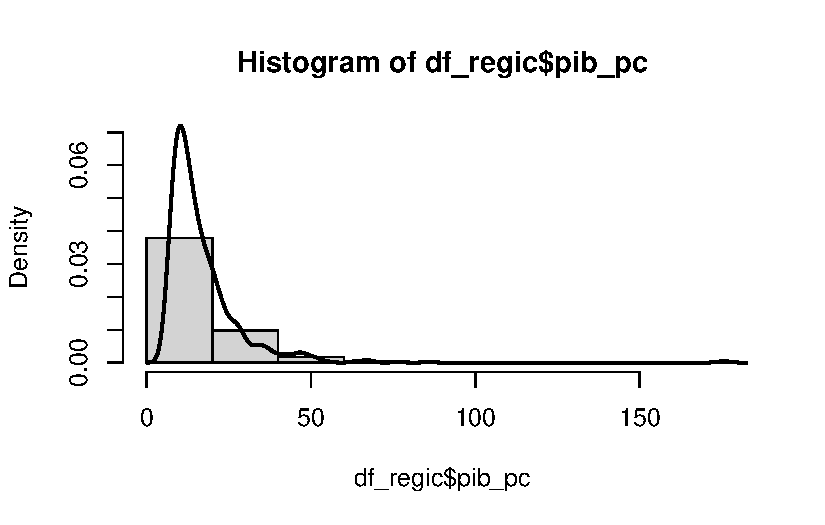
\includegraphics{main_files/figure-pdf/unnamed-chunk-3-1.pdf}

}

\end{figure}

\begin{Shaded}
\begin{Highlighting}[]
\FunctionTok{summary}\NormalTok{(df\_regic}\SpecialCharTok{$}\NormalTok{pib\_pc)}
\end{Highlighting}
\end{Shaded}

\begin{verbatim}
   Min. 1st Qu.  Median    Mean 3rd Qu.    Max. 
  5.388   9.945  13.484  17.128  19.856 177.101 
\end{verbatim}

\begin{Shaded}
\begin{Highlighting}[]
\FunctionTok{hist}\NormalTok{(df\_regic}\SpecialCharTok{$}\NormalTok{log\_cige, }\AttributeTok{freq=}\ConstantTok{FALSE}\NormalTok{)}
\FunctionTok{lines}\NormalTok{(}\FunctionTok{density}\NormalTok{(df\_regic}\SpecialCharTok{$}\NormalTok{log\_cige), }\AttributeTok{lwd=}\DecValTok{2}\NormalTok{)}
\end{Highlighting}
\end{Shaded}

\begin{figure}[H]

\caption{Coeficiente de Intensidade da Gestão Empresarial (CI)}

{\centering 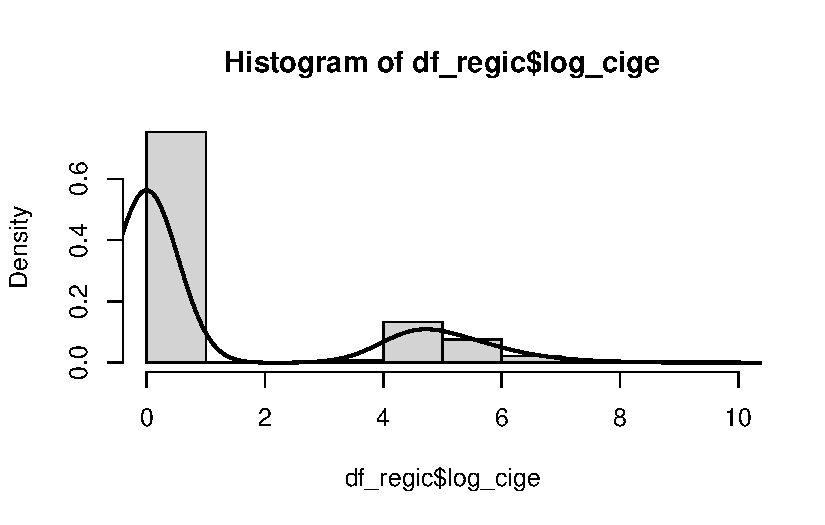
\includegraphics{main_files/figure-pdf/unnamed-chunk-5-1.pdf}

}

\end{figure}

\begin{Shaded}
\begin{Highlighting}[]
\FunctionTok{summary}\NormalTok{(df\_regic}\SpecialCharTok{$}\NormalTok{log\_cige)}
\end{Highlighting}
\end{Shaded}

\begin{verbatim}
   Min. 1st Qu.  Median    Mean 3rd Qu.    Max. 
  0.000   0.000   0.000   1.258   0.000   9.627 
\end{verbatim}

\begin{Shaded}
\begin{Highlighting}[]
\FunctionTok{hist}\NormalTok{(df\_regic}\SpecialCharTok{$}\NormalTok{log\_cgp, }\AttributeTok{freq=}\ConstantTok{FALSE}\NormalTok{)}
\FunctionTok{lines}\NormalTok{(}\FunctionTok{density}\NormalTok{(df\_regic}\SpecialCharTok{$}\NormalTok{log\_cgp), }\AttributeTok{lwd=}\DecValTok{2}\NormalTok{)}
\end{Highlighting}
\end{Shaded}

\begin{figure}[H]

\caption{Centralidade de Gestão Pública (CGP)}

{\centering 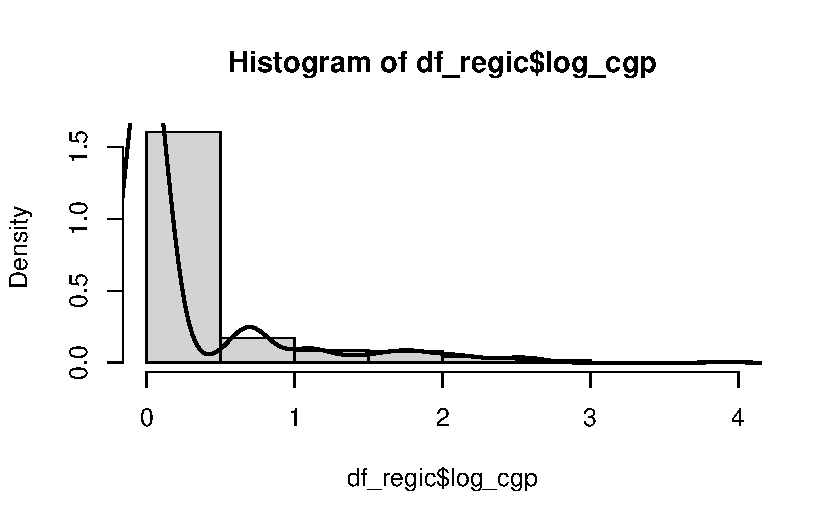
\includegraphics{main_files/figure-pdf/unnamed-chunk-7-1.pdf}

}

\end{figure}

\begin{Shaded}
\begin{Highlighting}[]
\FunctionTok{summary}\NormalTok{(df\_regic}\SpecialCharTok{$}\NormalTok{log\_cige)}
\end{Highlighting}
\end{Shaded}

\begin{verbatim}
   Min. 1st Qu.  Median    Mean 3rd Qu.    Max. 
  0.000   0.000   0.000   1.258   0.000   9.627 
\end{verbatim}

Heiss (2020) Greene (2019) (\textbf{Wooldrige?}) (\textbf{Hansen?})
\newpage

\hypertarget{referuxeancias}{%
\section{REFERÊNCIAS}\label{referuxeancias}}

\singlespacing

\hypertarget{refs}{}
\begin{CSLReferences}{0}{1}
\leavevmode\vadjust pre{\hypertarget{ref-greene}{}}%
GREENE, W. H.
\textbf{\href{http://gen.lib.rus.ec/book/index.php?md5=2BB86D2F4CF47DB0A519E94D262C3331}{Econometric
Analysis Global Edition}}. 8. ed. {[}s.l.{]} Pearson-prentice Hall,
2019.

\leavevmode\vadjust pre{\hypertarget{ref-heiss}{}}%
HEISS, F.
\textbf{\href{http://gen.lib.rus.ec/book/index.php?md5=5C3417608D22D155EA90339688548999}{Using
R for Introductory Econometrics}}. 2. ed. {[}s.l: s.n.{]}.

\end{CSLReferences}



\end{document}
